% Hubway Plots




%\begin{figure}
%	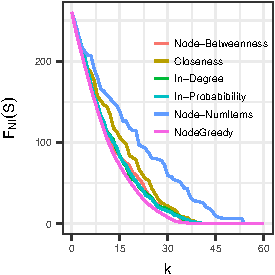
\includegraphics{figures/hubway_nodes.pdf}
%	\caption{Hubway node objective evolution.}
%	\label{fig:hubway_nodes}
%\end{figure}
%
%\begin{figure}
%	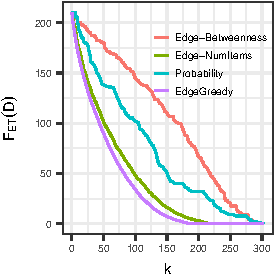
\includegraphics{figures/hubway_edges.pdf}
%	\caption{Hubway edge objective evolution.}
%	\label{fig:hubway_edges}
%\end{figure}


\begin{table*}[htbp]\small
\centering
\begin{tabular}{@{}llcccc@{}}
\toprule
\multirow{2}{*}{\begin{tabular}[l]{@{}l@{}}Graph\end{tabular}}                                                                         & \multirow{2}{*}{\begin{tabular}[l]{@{}l@{}}Item\\Distribution\ \ \ \ \ \ \end{tabular}} & \multirow{2}{*}{\begin{tabular}[l]{@{}l@{}}$r({\nodegreedy})$\end{tabular}} & \multirow{2}{*}{\begin{tabular}[l]{@{}l@{}}$r({\tt Node-Baseline}^\ast)$\end{tabular}} & \multirow{2}{*}{\begin{tabular}[l]{@{}l@{}}$r({\edgegreedy})$\end{tabular}} & \multirow{2}{*}{\begin{tabular}[l]{@{}l@{}}$r({\tt Edge-Baseline}^\ast)$\end{tabular}}\\ \\ \toprule
\multirow{4}{*}{\begin{tabular}[l]{@{}l@{}}{\autonomoussystems}\end{tabular}}  & {\ego}               & 0.06                                  & 0.24                                   & 0.14                                  & 0.15                                   \\
                                                                               & {\direct}            & 0.66                                  & 0.67                                   & 0.99                                  & 0.99                                   \\
                                                                               & {\uniform}           & 0.38                                  & 0.40                                   & 0.97                                  & 0.99                                   \\
                                                                               & {\inverse}           & 0.38                                  & 0.40                                   & 0.97                                  & 0.99                                   \\ \cmidrule(l){2-6}
\multirow{4}{*}{\begin{tabular}[l]{@{}l@{}}{\geo}\end{tabular}} 			   & {\ego}               & 0.00                                  & 0.06                                   & 0.01                                  & 0.02                                   \\
                                                                               & {\direct}            & 0.00                                  & 0.06                                   & 0.20                                  & 0.65                                   \\
                                                                               & {\uniform}           & 0.00                                  & 0.06                                   & 0.15                                  & 0.65                                   \\
                                                                               & {\inverse}           & 0.00                                  & 0.07                                   & 0.15                                  & 0.65                                   \\ \cmidrule(l){2-6}
\multirow{4}{*}{\begin{tabular}[l]{@{}l@{}}{\grid}\end{tabular}} 	           & {\ego}               & 0.27                                  & 0.27                                   & 0.29                                  & 0.29                                   \\
                                                                               & {\direct}            & 0.92                                  & 0.92                                   & 0.98                                  & 0.98                                   \\
                                                                               & {\uniform}           & 0.92                                  & 0.92                                   & 0.98                                  & 0.98                                   \\
                                                                               & {\inverse}           & 0.92                                  & 0.92                                   & 0.98                                  & 0.98                                   \\ \cmidrule(l){2-6}
\multirow{4}{*}{\begin{tabular}[l]{@{}l@{}}{\ba}\end{tabular}} 	               & {\ego}               & 0.18                                  & 0.56                                   & 0.26                                  & 0.26                                   \\
                                                                               & {\direct}            & 0.71                                  & 0.71                                   & 0.99                                  & 0.99                                   \\
                                                                               & {\uniform}           & 0.63                                  & 0.63                                   & 0.98                                  & 0.98                                   \\
                                                                               & {\inverse}           & 0.63                                  & 0.63                                   & 0.98                                  & 0.98                                   \\ \bottomrule                                                                             
\end{tabular}
\caption{Comparison of greedy algorithms with the best-performing baseline (${\tt Node-Baseline}^\ast$ and ${\tt Edge-Baseline}^\ast$) for $k=50$. 
For a given pair of graph and item-distribution scheme, $r(A)$ expresses the 
ratio of the expected uncertainty that algorithm $A$ achieves with $k=50$
monitoring operations over the initial uncertainty $\uncertainty_0$ 
(for $k=0$). Note that the best-performing baseline is different for different rows of the table.
}
\label{tab:objective-evolution-table}
\end{table*}

%\begin{table}[htbp]
%\centering
%\begin{tabular}{@{}ll@{}}
%\toprule
%ID & Landmark                           \\ \toprule
%33 & Kenmore Sq.                        \\
%36 & Copley Sq./Boston Public Library \\
%41 & Packard's Corner                   \\
%42 & Boston Public Garden               \\
%52 & Newbury St.                        \\ \bottomrule
%\end{tabular}
%\caption{Hubway stations in Boston city minimizing uncertainty (k=5).}
%\label{tab:hubway-table}
%\end{table}

% For both {\nodeproblem} and {\edgeproblem} problems, the number of items allocated to each node during initialization are chosen using three criteria,
% \begin{itemize} 
% 	\item Uniformly distributed over nodes.
% 	\item Directly proportional to the out-degree of the node.
% 	\item Inversely proportional to the out-degree of the node.
% \end{itemize}
% For each of the above three item initializations, we compare the following baseline approaches of choosing 'k' nodes,
% \begin{itemize}
% 	\item {\nodeproblem} baselines
% 	\begin{itemize}
% 		\item $k$ randomly chosen nodes.
% 		\item Top-$k$ nodes of highest incoming probabilities.
% 		\item Top-$k$ nodes of highest in-degree centrality scores.
% 		\item Top-$k$ nodes of highest degree-centrality scores.
% 		\item Top-$k$ nodes chosen using {\nodegreedy} algorithm.
% 	\end{itemize}
% 	\item {\edgeproblem} baselines
% 	\begin{itemize}
% 		\item $k$ randomly chosen edges.
% 		\item Top-$k$ edges of highest probabilities.
% 		\item Top-$k$ edges chosen using {\edgegreedy} algorithm.
% 	\end{itemize}
% \end{itemize}
% For each of the configurations described above, we make following two plots,
% \begin{itemize}
% 	\item Evolution of objective function value for $k=0$ over time. (At some time, the items distribution over nodes approaches the stationary distribution. The objective function value for $k=0$ remains constant thereafter.)

% 	\item Evolution of objective function value over different values of $k$. (As the $k$ increases, the uncertainty should decrease ultimately to zero.)

% \end{itemize}



\begin{figure}
\begin{subfigure}[b]{0.23\textwidth}
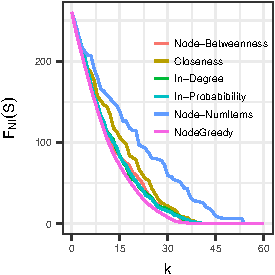
\includegraphics[width=\textwidth]{figures/hubway_nodes.pdf}
\caption{{\nodeproblem}}
\label{fig:hubway_nodes}
\end{subfigure}
\begin{subfigure}[b]{0.23\textwidth}
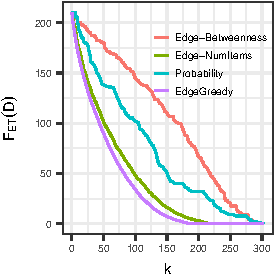
\includegraphics[width=\textwidth]{figures/hubway_edges.pdf}
\caption{{\edgeproblem}}
\label{fig:hubway_edges}
\end{subfigure}
\caption{{\hubway} data; $y$-axis: expected uncertainty, $x$-axis: number of monitored nodes or edges.}
\end{figure}



\subsection{Experimental results}
In this section, we report the   
performance of algorithms for the {\mcproblem} problem -
first on the graph datasets, combined with item distribution schemes;
then on the \hubway\ dataset.
As objective we always use the expected uncertainty
achieved for a given budget $k$ of nodes or edges -- the smaller its value,
the better the performance of the algorithm.
Note that we do not report separately the performance of \edgeDP, as it achieves
same performance as \edgegreedy, but is not as efficient.


We provide the results for the graph datasets in Table \ref{tab:objective-evolution-table}. 
In all these experiments we use $k=50$.
Moreover, $r(A)$ is the ratio of the achieved objective value (for $k=50$) over
the initial value $\uncertainty_0$ of the measure 
(for no monitoring operations, i.e., $k=0$).
The table shows four quantities for every graph-item distribution pair
: $r(A)$ for $A=\{${\nodegreedy}, {\tt Node-Baseline}$^\ast$, {\edgegreedy}, {\tt Edge-Baseline}$^\ast$ $\}$.
Note that {\tt Node-Baseline}$^\ast$ (resp.\ {\tt Edge-Baseline}$^\ast$) refers to the baseline 
algorithm with the best performance.
For every algorithm $A$, $r(A)\in[0,1]$ and the smaller the value of $r(A)$ the better the performance of the algorithm.
 
From the table, we observe that for 
the {\autonomoussystems} dataset,  {\nodegreedy}  significantly outperforms the best
baseline for the {\ego} item distribution, while performing marginally better for other item distributions.
The value of  $r({\edgegreedy})$ is only slightly less than
the best baselines across all the configurations. However, we observe that there is no baseline
which performs uniformly the best across different item distributions. For example,  {\edgebetweenness}
is the best baseline for {\direct} item distribution, the {\edgenumitems} for {\ego}, while they both
perform worse than even randomly chosen edges for {\uniform} and {\inverse} item distributions.
Notably, for the {\geo} graphs, the greedy algorithms significantly outperform the baselines


For the {\grid} graphs, the baselines perform exactly
the same as our algorithms. This can be explained by the nature of the 
{\grid} graph, where all the nodes except the ones on the boundary are similar to each other,
thereby rendering the {\direct}, {\uniform} and {\inverse} item distributions very similar 
to each other. For the {\ego} distribution, the greedy algorithms perform marginally better
than the baselines.
%, depending on the number of nodes within the fixed radius around the randomly chosen node, 
%and the percentage of items distributed among these nodes. 
Again,
there is no baseline which performs uniformly the best.
Similar is our explanation for the results on {\ba} graphs as in these graphs most of the nodes have
almost the same (small) degrees too.

A more thorough investigation of the performance of the algorithms for different
values of $k$ and for all datasets we consider is shown in 
Supplementary Material, Section~\ref{sec:additional_results}.





\spara{Experiments with {\hubway} data:}
In our last experiment, 
we explore the performance of our algorithms on the {\hubway} dataset. From Figure \ref{fig:hubway_nodes}
and Figure \ref{fig:hubway_edges} we observe that the {\nodegreedy} and {\edgegreedy} algorithms
are consistently the best at reducing expected uncertainty, although the baselines are competitive on the
relatively smaller graph. In Figure \ref{fig:hubway_stations}, we plot the Hubway stations across Boston
chosen by the {\nodegreedy} algorithm with $k=5$. The nodes chosen by the algorithm are supported by
the anecdotal evidence of being exactly some of the of the most popular landmarks around the city.
From a managerial perspective, tracking the number of trips starting or ending at these Hubway stations
can help the operators better reduce the expected uncertainty around the expected number of bikes
available at its different stations and anticipate future bike ``re-balancing"\footnote{https://www.citylab.com/transportation/2014/08/balancing-bike-share-stations-has-become-a-serious-scientific-endeavor/379188/} operations.

\spara{Running times:} For all our experiments we use a single process 
implementation of our algorithms on a 24-core 2.9GHz Intel Xeon E5 processor 
with 512GB memory. For the  largest graph in our experiments,  
the parallelized version of the {\nodegreedy}\ takes about $5-10$ 
seconds per selected node, while the parallelized version of {\edgegreedy}\ 
takes about $1$ minute per selected edge.

\begin{figure}
	\centering
	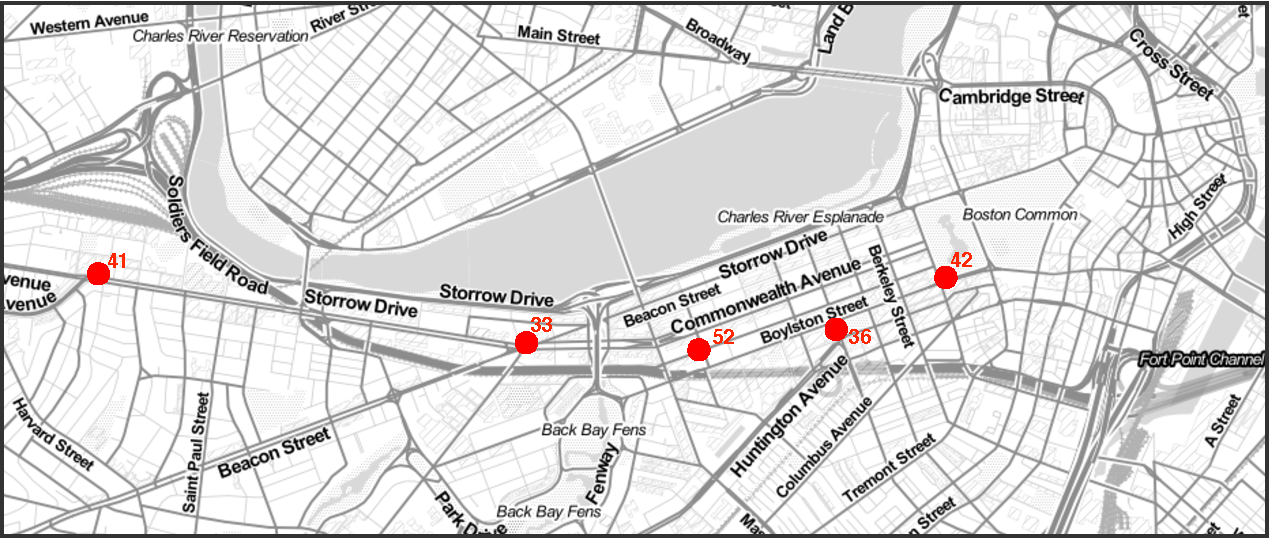
\includegraphics[width=8cm, height=4cm]{figures/hubway_stations_5.pdf}
	\caption{{\hubway} data. IDs of stations picked as a solution to {\nodeproblem}
	for $k=5$;
	33: Kenmore Sq., 36: Copley Sq./Boston Public Library, 41: Packard's Corner, 
	42: Boston Public Garden, 52: Newbury St.                        }
	\label{fig:hubway_stations}
\end{figure}


\spara{Discussion:} Our experiments show that  {\nodegreedy} and  {\edgegreedy} 
consistently perform better than or on par with other popular baseline methods. Also, for 
graphs with relatively large number of nodes, the solutions to the {\nodeproblem} problem 
are more effective at reducing
the expected uncertainty than the solutions to the {\edgeproblem} problem for the same number of
node (resp.\ edge) monitors.
This is
especially important considering our analysis from Section \ref{sec:nodes} and \ref{sec:edges} which show
that the {\nodegreedy} algorithm has a better time complexity compared to the {\edgegreedy} for dense graphs.

